\documentclass{article}
\usepackage{graphicx} % Required for inserting images
\usepackage{graphicx, centernot, amsmath, bbm, booktabs, multirow, array, capt-of, varwidth, natbib, amstext, tabularx}
%\DeclareMathOperator{\E}{\mathbb{E}}

\usepackage[utf8]{inputenc}
\usepackage{dirtytalk}
\usepackage{csquotes}
\usepackage{graphicx}
\usepackage{amsmath,amsthm,amsfonts}
\usepackage{lipsum}
\usepackage[utf8]{inputenc}
\usepackage{hyperref}
\usepackage{float}
\hypersetup{
    colorlinks=true,
    linkcolor=blue,
    filecolor=magenta,      
    urlcolor=cyan,
    pdftitle={Overleaf Example},
    pdfpagemode=FullScreen,
    }
\usepackage{tikz}
\usetikzlibrary{bayesnet}
%\newcommand{\thought}[1]{{\color[rgb]{0.2,0.39,0.66}(#1)}}
\newcommand{\todo}[1]{{\color[rgb]{1.0,0.0,0.0}(#1)}}
\newcommand{\hsh}[1]{{\color{green!50!black} Henrik: #1}}
\newcommand{\st}[1]{{\color{red!50!black} Sebastian: #1}}

\newcommand{\ulm}[1]{_{\scaleto{\mathrm{#1}}{3pt}}}
\newcommand\at[2]{\left.#1\right|_{#2}}











\newtheorem{assumption}{Assumption}

\DeclareMathOperator*{\argmax}{arg\,max}
\DeclareMathOperator*{\argmin}{arg\,min}

\newcommand{\swname}[1]{\texttt{#1}}
\newcommand{\ie}{i\/.\/e\/.,\/~}
\newcommand{\eg}{e\/.\/g\/.,\/~}
\newcommand{\cf}{cf\/.\/~}

\newcommand{\fig}{Fig\/.\/~}
\newcommand{\defn}{Def\/.\/~}
\newcommand{\sect}{Sec\/.\/~}
\newcommand{\tabl}{Tab\/.\/~}
\newcommand{\algo}{Algorithm~}
\newcommand{\theo}{Theorem~}

\newcommand{\bnnl}{3 hidden layers}
\newcommand{\bnnn}{50 neurons}
\newcommand{\bnna}{tanh activations}

\newcommand{\capt}[1]{\mdseries{\emph{#1}}}

\newcommand{\videolink}{at \url{https://youtu.be/_d7AqTRjz6g}}
\newcommand{\codelink}{\url{https://github.com/wheelbot/mini-wheelbot}}

\newcommand{\fakepar}[1]{\vspace{0mm}\noindent\textbf{#1.}}

\newcommand{\needref}{\textcolor{red}{[REF]}}

\newcommand{\plotfontsize}{9pt}


\newcommand{\ours}{$\text{Q}$LASS}
%\documentclass{article}
%\usepackage[demo]{graphicx}
\usepackage{caption}
\usepackage{subcaption}

\title{Designing Experimental Evaluations 
of Algorithmic Interventions 
with Human Decision Makers In Mind}
% Previous: Auditing Algorithmic Interventions
\author{Deb Raji, Lydia Liu}
\date{March 2024}

\begin{document}


\maketitle
\begin{abstract}

 Automated decision systems (ADS) are broadly deployed to inform or support human decision-making across a wide range of consequential contexts. An emerging approach to the assessment of such systems is through experimental evaluation, which aims to measure the causal impacts of the ADS deployment on decision making and outcomes. However, various context-specific details complicate the goal of establishing meaningful experimental evaluations for algorithmic interventions. Notably, current experimental designs rely on simplifying assumptions about human decision making in order to derive causal estimates. In reality, cognitive biases of human decision makers \emph{induced} by the experimental design may significantly alter the observed effect sizes of the algorithmic intervention.
 In this paper, we formalize and investigate various models of human decision-making in the presence of a predictive algorithmic aid. We show  that each of these behavioral models produces dependencies across decision subjects and results in the violation of existing assumptions, with consequences for treatment effect estimation. 
This work aims to further advance the scientific validity of intervention-based evaluation schemes for the assessment of algorithmic deployments, by exploring the ways in which the current available evidence for such interventions falls short of providing conclusive findings. 
\end{abstract}

\section{Introduction}

In particular, we examine the role of specific \emph{experiment design choices} in judge responsiveness -- specifically, choices that experiment designers make on the treatment assignment model ($Z$), the positive prediction rate  ($P (\hat{Y} = 1)$) (by setting the threshold of the model with respect to recommended action) and the model correctness ($P (\hat{Y} = Y)$) (through model selection).

We argue that these experiment design choices impact the natural deviation and automation bias of the judges relying on algorithmic recommendations, which in turn distorts our understanding of the average treatment effect of algorithmic interventions. 

\begin{itemize}
    \item Context: social institutional decision-making 
    \item data($X$) $\rightarrow$ prediction ($\hat{Y}$) $\rightarrow$ decision ($D$) $\rightarrow$ outcome ($Y$); 
    \item Note: ~\cite{kleinberg2018human} presents: data($X$) $\rightarrow$ prediction ($\hat{Y}$) $\rightarrow$ decision ($D$)
    \item Note that outcomes can be observed proxies or direct measurement of downstream outcomes
\end{itemize}

Experiment design often boils down to the following main choices:
\begin{itemize}
    \item Treatment assignment model
    \begin{itemize}
        \item Proportion of units treated ; two-level randomization \cite{crepon2013labor}
        \item method of participant allocation to experimental group 
        \item treatment assignment model 
    \end{itemize}
    \item Power -- number of units included in experiment
    \item Type of treatment 
\end{itemize}

We believe these choices impact the decision-making of the judge in important ways, and that the deviation of the judge from algorithmic recommendation is not just an inherent feature of that judge but also in response to experiment design choices. 

\section{Related Work}

\subsection{Experimental evaluations of algorithmic interventions}

Here we focus the following case study~\cite{imai2020experimental}. 

During a 30-month assignment period, spanning 2017 until 2019, judges in Dane County, Wisconsin were either given or not given a pretrial Public Safety Assessment (PSA) score for a given case. The randomization was done by an independent administrative court member - the PSA score was calculated for each case $i$, and, for every even-numbered case, the PSA was shown to the judge $k$ as part of the case files. Otherwise, the PSA was hidden from the judge. Given these scores, the judge needs to make the decision, $D_{i,k}$ to enforce a signature bond, a small case bail (defined as less than \$1000) or a large case bail (defined as more than \$1000). Information about judge decisions, and defendant outcomes, $Y_{i,k}$ (ie. failure to appear (FTA), new criminal activity (NCA) and new violent criminal activity (NVCA)) are tracked for a period of two years after randomization. 

The case study~\cite{imai2020experimental} only looks at one judge, allowing them to simplify the situation to a single decision-maker scenario. Thus, in this study, the assumed causal relationships between variables can thus be simplified to Figure 2. %~\ref{imai_diagram}. 


%The main analytical 

%subsequent data on FTA, NCA, NVCA, and other outcomes for a period of two years after randomization

The causal question is in determining how the treatment of providing PSA scores for a given case impacts the decision being made by the judge, and the supposed \emph{correctness} of that decision. Assumption 4 (Exclusion Restriction) in the case study ~\cite{imai2020experimental} states that ``the provision of the PSA influences the outcome only through the judge’s decision'', meaning that cases do not influence each other -- an outcome that reasonably holds since each case analyzed is the first case of the considered defendant. However, there is no meaningful discussion of how decisions might be confounded, beyond an assessment of a minimal ~\emph{spillover effect}~\cite{sinclair2012detecting}, by demonstrating that the order of case appearance does not seem to impact the judge's decisions. 

The authors state that it should be optimal for the judge to be more lenient for lower risk cases, and harsher for higher risk cases - this leads them to stratify the treatment effect analysis by risk level ( i.e. "preventable cases", "risky cases" and "safe cases"). They determine a set of assumptions then define the following average principal causal effect (APCE) for various risk levels:

$$ APCE = E\{ D_i(1) - D_i(0) | Y_i(1) = y_0, Y_i(0) = y_i\}$$

Where $ D_i(1)$ is the decision under treatment $Z_i$ and $Y_i(1)$ are the outcomes under treatment. $D_i(0)$ and $Y_i(0)$ mean $Z_i = 0$ and these are the results under no treatment. $y_0$ and $y_i$ are $\in \{0,1\}$. When $(y_0,y_i) = (0,1)$, then it is a preventable risk, meaning for example, an NCA occurs if released. When $(y_0,y_i) = (1,1)$, the outcome would happen regardless of release and when $(y_0,y_i) = (0,0)$, the outcome would not occur regardless of release. 

The main empirical result is that when looking at average treatment effects on judge decisions and downstream outcomes, there is a negligible impact of the PSA provision on the judges' overall decision-making. As a result, there were also not many notable differences in downstream outcome.  

Interestingly, the authors conclude that there are meaningful demographic differences with respect to gender - ie. the analysis concludes that making the PSA visible leads to more lenient decisions for female defendants, while male defendants are relatively unaffected. Similarly, the PSA provision does not seem to have a significant disparate impact due to race. 

\subsubsection{Modeling human decision-making in the presence of algorithmic interventions}
%simulation // ben green 

In ~\cite{albright2019if}, Albright assesses observational case-level data sourced from the Kentucky Administrative Office of the Courts, before and after a certain Kentucky policy change on June 8, 2011-  House Bill 463 (HB463). The policy requires judges to more actively factor in the assessment score level (high, moderate and low), as calculated by the Kentucky Pretrial Risk Assessment (KPRA), in their decision-making. They were requested to release all low and moderate risk defendants with a non-financial bond, unless actively providing justification for their deviance. 

The author begins by simply analyzing trends in the available data, collected from 2009 to 2013. They determine that there is an observed discontinuous jump in the percentage of non-financial bonds provided in the period after the implementation of the policy. To be precise - for male defendants, the mean of the percentage of non-financial bonds jumped from pre-HB463 levels of 22.5\% to post-HB463 levels of 36.5\%. The authors then dis-aggregate results by race, finding that this impact is disproportionately visible for White defendants, and low risk defendants. They conclude that although the explicit consideration of the risk score via HB463 overall leads to more leniency in judge decision-making, the scores have little to no effect on high risk defendant decisions of any race and Black defendants in general. 

The authors look at the distribution of risk scores by race, similar to the analysis done on COMPAS risk scores ~\cite{angwin2016machine}. What they find is a much milder picture - the distribution across races are much more similar, though white defendants are still slightly more skewed towards the lower-risk levels. This discrepancy is not so great, however, to account for a meaningful difference in bond decisions - racial disparities are thus most evident in the deviations from the risk score recommendation when HB463 requires the risk score to be considered (ie. for low and moderate risk). 


This quasi-experimental setting creates the possibility of a difference in differences study taking advantage of the implementation of HB463 as a natural experiment in examining the impact of the introduction of the use of the KPRA score on the decision of judge $j$ to set a non-financial bond ($b_{ictj} = 1$) or not ($b_{ictj} = 0$) for defendant $i$ with charges $c$ at time $t$. We are interested in the impact of the race of the involved defendants before and after the policy change. So, we introduce $HB463_t$ as an indicator of whether the decision takes place before or after the effective data of HB463, and $Black_i$ as an indicator of whether or not the defendant is Black. $\delta_i$ is a vector of defendant characteristics to control for (ie. age, criminal history, dummy variables for prior convictions, pending cases, etc.) and  $\kappa_c$ is a vector of charge-related dummy variables (ie. charge levels, charge letter classes, etc.). $\omega_{j}$ is judge fixed-effects, meant to represent differences in judge-specific decision rules. $x_t$ represents temporal effects, ie. month-year fixed effects.

The modeled relationship is thus theorized in the following equation:

$$ b_{ijct} = \alpha + \phi_1 HB463_t + \phi_2 Black_i + \phi_3(Black_i \times HB463_t) + \beta_1\kappa_c + \beta_2 \delta_i + \omega_{j} + x_t + \varepsilon_{ijct} $$

The co-efficient of interest is thus $\phi_3$, indicating the change in the racial gap in the issuance of non-financial bonds, following the implementation of HB463. 

The main results reveal that pre-HB463, differences between Black and White defendants is negligible. However, post-HB463, white defendants receive a significantly greater amount of leniency, experiencing 30\% and 62\% more of the short-term gains in non-financial bonds than their Black counter-parts in low and moderate risk score settings. Even when adjusting for time-dependent judge-fixed effects,  $\omega_{jt}$, Black defendants still experience a 25\% lower increase in non-financial bond issuance. 

\subsubsection{Case Study \# 3}

The next case involves the setting of hiring managers ~\cite{hoffman2018discretion}. 

Here, the goal is to optimize the match quality E[a|Hire]. 



\subsubsection{Case Study \# 4}

We also analyze the case of the use of  of risk assessments in the medical setting~\cite{mullainathan2022diagnosing}. 

In this context, they differentiate between a ``socially optimal'' and "physician" decision thresholds for testing. 

Physician bias is impacted by the following:
\begin{itemize}
    \item \textbf{Boundedness of Physician judgements}
    This entails looking at a subset of number of variables of X, because analyzing the full scope of $X_ij$ is not likely. 
    They model the decisions as $m_{simple}(X_ij)$ 
    \item \textbf{Biases}
    Here we look (over- or under-weighing certain variables)
    \item Representativeness 
\end{itemize}





\section{Current paradigm and assumptions}

We are interested in the problem of experimentally evaluating how algorithmic interventions in the form of predictive decision aids influence human decision-making. In this section, we describe the existing paradigm for experimental evaluations---we call this the \emph{case-independent} model---and the common assumptions required for causal identification. 

 In many existing experimental evaluations of algorithmic decision aids, the \emph{treatment unit} is presumed to be the decision subject and the \emph{treatment}, $Z_i$ is conceptualized as the provision of an predictive risk score to a decision maker who is responsible for making the final decision $D_i$. In the case of pre-trial detention decisions, the decision subject is the defendant in a particular court case, the decision maker is the judge presiding on the case, and the treatment $Z_i$ is a binary variable indicating if the PSA is shown to the judge for case $i$. $D_i$ represents the judge's binary detention decision, where $D_i = 1$ means detaining and $D_i = 0$ means releasing the arrestee before trial. $Y_i$ is the binary outcome variable, with $Y_i = 1$ indicating the arrestee committed an NCA, and $Y_i = 0$ indicating they did not. $X_i$ is a vector of observed pre-treatment covariates for case $i$, including age, gender, race, and prior criminal history. Independence is assumed between each case. We illustrate these variables and their dependencies (or lack thereof) in Figure~\ref{fig:indep_causal_model}.

 
 \begin{figure}[htbp]
  \centering
 \includegraphics[trim=1.5cm 2cm 3cm 10cm, clip, width=\columnwidth]{alg_int_neurips24_bw_imai_simple.pdf}
  \caption{The case-independent model of human decision making with a predictive decision aid. This is the causal model assumed in prior work \citep[e.g.,][]{imai2020experimental}}
  \label{fig:indep_causal_model}
\end{figure}

The crucial assumption here is that of non-interference between treatment units (see Assumption~\ref{assmp:sutva}, SUTVA). In words, the treatment status of one unit should not affect the decision for another unit. As a result, $Z_i$ is typically randomized at a single-level, i.e., on individual cases; and there is no randomization at the level of decision makers. %This means that, for a random selection of cases, the algorithmic recommendation or result is shown to the corresponding decision-maker. 
In \citet{imai2020experimental} for example, where only one judge participated in the study, the algorithmic score is shown only for cases with an even case number (i.e., $Z_i =1$); for odd-numbered cases, no algorithmic recommendation is shown (i.e., $Z_i =0$). 

The assumption of non-interference across units is debatable and unlikely to hold, for multiple reasons. For one, in the psychology and behavioural economics literature, it is well-known that decision-makers have a bias towards consistency to their internal policies for decision-making and generally do not change on a case by case basis~\cite{tversky1985framing}. What this means is that, in ~\cite{imai2020experimental} for example, where the judge only sees the risk score for a fraction of the cases, they might choose to ignore the PSA completely on cases where they do see it or to infer patterns for cases where they don’t see the score, in order to be as consistent as possible in their decision-making (in this work, we mainly model effects such as the former). %Such case-based interventions thus allow for only a \emph{\textbf{partial treatment for the decision-makers under case randomization}}.
 
 Other work have considered hetereogeneity across decision makers, though they assume that the tendency to follow or not follow the recommendation based on an algorithmic score is inherent to each judge---an inherent attribute of the judges' internal state or their access to privileged decision and factors outside of the experimenter's control. In \citet{hoffman2018discretion}, which studied decisions made by hiring managers with a decision aid, they consider possible access to privileged information that impacted the hiring manager's judgement (and considers each hiring manager to have a particular \emph{exception rate} for making a different decision from the algorithm). \citet{angwin2016machine} discussed the cost $\eta$ of deviation, since the judge has to actively log deviations from the algorithmic recommendation. In both of these cases, judge responsiveness is defined as a factor of the environment or as an intrinsic feature of the judge---in other words, factors that the experimenter cannot control. In the next section, we describe our model of judges and use it to demonstrate how design decisions about the experiment can impact judge responsiveness in ways that will impact downstream average treatment estimates. 

 %Spillover effect measured by randomizing the cases 


\iffalse
\begin{figure}[H]
    %\label{imai_diagram}
	\centering	
	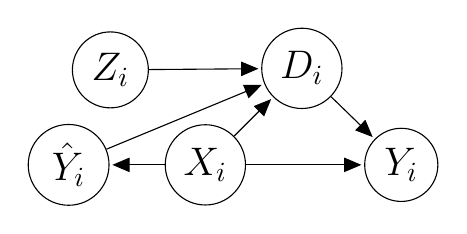
\begin{tikzpicture}[->,shorten >=1pt,auto,node distance=2cm,
	main node/.style={circle,draw,font=\Large}]
	
	\node[main node] (T1) {$X_{i}$};
	\node[main node] (X1) [above right =7mm of T1]{$D_{i}$};
	%\node[main node] (X1pre) [above left =1cm of X1]{$J_k$};
    %\node[main node] (Z1) [left =1cm of X1pre]{$Z_k$};
   \node[main node] (Z2) [above left = 7mm of T1]{$Z_{i}$};
	\node[main node] (Y1) [right=1.5 cm of T1] {$Y_{i}$};
  \node[main node] (P1) [left =7mm of T1]{$\hat{Y}_{i}$};
	
	%\plate [inner sep=.25cm,yshift=.2cm] {plate1} {(X1pre)(X1)(Y1)(T1)(Z1)} {$i$}; 
	
	\path[every node/.style={font=\small}]
	(X1) 	edge node [right] {} (Y1)
  %  (Z1) edge node [right] {} (X1pre)
	%(X1pre) edge node [right] {} (X1)
    (Z2) edge node [right] {} (X1)
    %(Z2) edge node [right] {} (X1pre)
    (T1) edge node [right] {} (P1)
    (P1)edge node [right] {} (X1)
	(T1) edge node [right] {} (Y1)
	edge node [right] {} (X1);
	\end{tikzpicture}
		\caption{Proposed causal model in case study ~\cite{imai2020experimental}}
\end{figure}
\fi


 
 
 % Therefore, we can’t draw clear conclusions on how the judge modifies their default policy in response to the algorithm, since we don’t observe the fully algorithmically modified policy for a given case. Note that is distinct from the known phenomenon of spillover effects, which highlight how case order can impact judgement on the next case. With partial treatment, even when order does not matter, all cases are judged differently from the expected treatment, due to the bias of the decision-maker towards consistency. In this case, the consequence of this partial treatment is likely an under-estimation in the impact of a full treatment. We need the execution of the intervention to actually operate as a binary treatment (ie. $Z_{i,k} \in \{1, 0\}$) in order to satisfy the assumptions of SUTVA. 



%\textbf{Ideas for theory:}
%        \begin{itemize}
%            \item Model the Judge's internal state $J_k$ (this could be the weight they place on PSA in decision) as changing over time (e.g. with more exposure to PSA). $J_k$ could be an explicit function of the likelihood of seeing a PSA.
%            \item Use this model to show that order of the cases does not matter for treatment effect (for this need to understand how the conditional independence/ permutation test in \cite{imai2020experimental} works), but still the treatment effect is underestimating the true treatment effect under total treatment, i.e. $Z_{i,k} = 1 \forall i$ where case $i$ is matched to judge $k$.
%        \end{itemize}

To address the partial treatment for decision-makers under case randomization, there are various approaches to explore. One approach to this issue could be to model the Judge's internal state $J_k$ (e.g. this could be the weight they place on PSA in decision) as changing over time (e.g. with more exposure to PSA). $J_k$ could be an explicit function of the likelihood of seeing a PSA. We can then use this model to show that the order of the cases does not matter for determining the treatment effect, but that the measured treatment effect is likely underestimating the true treatment effect under total treatment, i.e. $Z_{i,k} = 1 \forall i$ where case $i$ is matched to judge $k$.
 
    
        %In ~\cite{albright2019if}, the analyzed policy only requires the active consideration of risk scores at the low and medium level - at high levels, judges are still able to ignore the scores. It is clear that, to some level, when given the option, the judges do seem to ignore the scores - the implementation of the policy had no to little impact on decision-making for judges on high risk cases. 
        
        %re is almost no impact to the judge decisions before the implementation of the policy for high risk score defendants, because the policy 
        %which the authors measure as insignificant, ie. order of presentation of PSA/no-PSA does not matter. 
        
It is also note-worthy that the analyzed quasi-experimental investigations also involve only case-level analysis of the data~\cite{albright2019if, hoffman2018discretion}. However, ~\cite{albright2019if} does include some consideration of judge-specific impacts through the inclusion of time-dependent fixed-judge effects in their analysis (see Appendix A). What they found is that the judge-specific impacts were significant and worth investigating further - in particular, racial disparities for low risk defendants seemed to be driven specifically by variance across judges.
 



\section{Model}
In this section, we propose a novel causal model of algorithm-aided human decision making that is distinct from case-independent model, as depicted in Figure~\ref{fig:indep_causal_model}. Our model, depicted as a causal directed acyclic graph (Figure~\ref{fig:expanded_causal_model}), accounts for dependence in the decisions across cases induced by the human decision maker's cognitive bias. We consider three types of cognitive bias that are particularly relevant to the current setting of human decision making with a predictive decision aid---all of which are directly influenced by experimental design choices (Table~\ref{table:cognitive_bias_models}). We do so by introducing two latent variables $J_{i,k}$ and $\epsilon_{i,k}$ that track the internal state of the decision maker $k$ and how it affects the decision for subject $i$.

\begin{figure}[htbp]
  \centering
  \includegraphics[trim=1.5cm 2cm 3cm 6cm, clip, width=\columnwidth]{alg_int_neurips24_bw.pdf}
  \caption{Proposed causal model that accounts for human decision maker bias. We describe three versions of this model (see Table~\ref{table:cognitive_bias_models}). Under the \emph{treatment exposure} model, arrow (i) is activated, but not (ii) and (iii). Under the \emph{capacity constraint} model, arrows (i) and (ii) are activated, but not (iii). Under the \emph{low trust} model, all three arrows, (i-iii), are activated.}
  \label{fig:expanded_causal_model}
\end{figure}

\iffalse
\begin{figure}[H]
	\centering	
	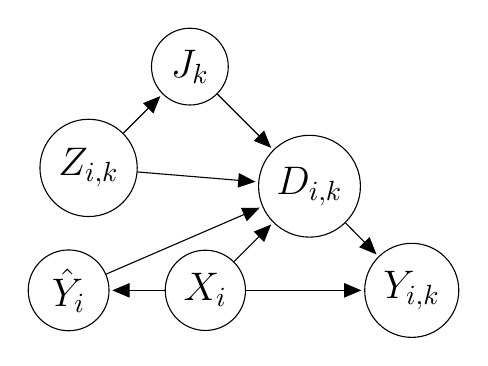
\begin{tikzpicture}[->,shorten >=1pt,auto,node distance=2cm,
	main node/.style={circle,draw,font=\Large}]
	
	\node[main node] (T1) {$X_{i}$};
	\node[main node] (X1) [above right =7mm of T1]{$D_{i,k}$};
	\node[main node] (X1pre) [above left =1cm of X1]{$J_k$};
 %\node[main node] (Z1) [left =1cm of X1pre]{$Z_k$};
   \node[main node] (Z2) [below left = 7mm of X1pre]{$Z_{i,k}$};
	\node[main node] (Y1) [right=1.5 cm of T1] {$Y_{i,k}$};
  \node[main node] (P1) [left =7mm of T1]{$\hat{Y}_{i}$};
	
	%\plate [inner sep=.25cm,yshift=.2cm] {plate1} {(X1pre)(X1)(Y1)(T1)(Z1)} {$i$}; 
	
	\path[every node/.style={font=\small}]
	(X1) 	edge node [right] {} (Y1)
  %  (Z1) edge node [right] {} (X1pre)
	(X1pre) edge node [right] {} (X1)
    (Z2) edge node [right] {} (X1)
    (Z2) edge node [right] {} (X1pre)
    (T1) edge node [right] {} (P1)
    (P1)edge node [right] {} (X1)
	(T1) edge node [right] {} (Y1)
	edge node [right] {} (X1);
	\end{tikzpicture}
		\caption{Proposed full causal model}
\end{figure}
\fi 

As in the case-independent model, we assume that $X_i$'s are independent and identically distributed.
In contrast to the case-independent model that does not include the role of the human decision maker (i.e., the judge), we explicitly model the judge---we index each case decision $D_{i,k}$ by both the decision maker (index $k$ in Figure~\ref{fig:expanded_causal_model}) and the decision subject (index $i$ or $\ell$ in Figure~\ref{fig:expanded_causal_model}), as opposed to only indexing it by the decision subject. Similarly, the treatment assignment variable $Z_{i,k}$ denotes the treatment status of both the decision subject $i$ and the decision maker $k$. This provides a fuller account of the space of possible treatment assignment counterfactuals, e.g., a case could have been assigned to a different judge leading to a different decision and outcome, all else held constant. 
We further assume that the judge is sequentially exposed to cases, where the judges consider case $i$ after the case $i-1$, and one case at a time.

To be precise, we define
\begin{equation*}
    Z_{i,k}
 = 
\begin{cases}
1 \text{ if unit } i \text{ is assigned to Judge }k \text{ and unit } i \text{ received algorithmic treatment}\\
0 \text{ if unit } i \text{ is assigned to Judge }k \text{ and unit } i \text{ received no treatment} \\
-1 \text{ if unit } i \text{ is not assigned to Judge }k 
  \end{cases}
\end{equation*}  

As the decision outcome $Y_{i,k}$ is downstream of $D_{i,k}$, we also index it by both the judge and the decision subject.

\subsection{Judge's decision}\label{sec:judge_dec}


We model the judge's decision for each treatment unit in the experiment as a random event, whose probability is determined by the individual judge's decision parameters as well as aspects of the experimental design (e.g. the treatment assignments).

We assume that for each judge $k$, there exists a default decision function (in absence of any algorithmic decision aid) $\lambda_k$ that takes in observable characteristics $X_i \in \calX$. When no predictive decision aid is provided to the unit $i$ assigned to judge $k$ (i.e., $Z_{i,k} = 0$), the judge follows her default decision process and her decision $D_{i,k}$ takes value $\lambda_k(X_i)$.

Suppose, instead, that the unit $i$ is treated (i.e., $Z_{i,k} = 1$). In this case, the judge is provided with the algorithmic score $\hat{Y}_i$. We denote as $\bar{D}(y)$ the recommended decision function mapping a prediction $y$ to a decision (this models, for example, existing judge decision guidelines for PSA scores).

In the case that $\recdec{i}$ differs from the judge's default decision $\lambda_k(X_i)$, the judge may choose to `comply' with the $\recdec{i}$, or to disagree with the ADS recommendation and choose $\lambda_k(X_i)$. We model this as a random event as follows. Let $J_{i,k}$ denote the \emph{responsiveness} of Judge $k$ for treatment unit~$i$, i.e. the probability that the Judge follows the PSA recommendation for case $i$. In other words, $J_{i,k}$ models the automation bias of the judge at the point they are deciding on unit $i$. Let $\epsilon_{i,k} \sim Ber(J_{i,k})$ be the random variable denoting judge response, drawn independently for each $i$; when $\epsilon_{i,k} = 1$, the judge  `complies' with the ADS recommendation. 

To summarize, we have the following decision for judge $k$ on unit $i$:
\begin{equation*}
    D_{i,k} = \begin{cases}
        \lambda_k(X_i) \text{ if } Z_{i,k} = 0 \text{ (no PSA) } \\
        \begin{cases}
     \recdec{i} &\text{if } \recdec{i} = \lambda_k(X_i)  \text{ or } \epsilon_{i,k}=1 ~\text{(Judge complies)}\\
        \lambda_k(X_i) &\text{if }\recdec{i} \ne \lambda_k(X_i) \text{ and } \epsilon_{i,k}=0 ~\text{(Judge does not comply)}
      %  \recdec{i} & \text{o.w.} %&\text{ w.p. $J_k$}
        \end{cases} \text{o.w.}
    \end{cases}.
\end{equation*}
Equivalently:
\begin{equation}\label{eq:model_of_judge}
    D_{i,k} = \left( \bar{D}(\hat{Y}_i)\cdot \epsilon_{i,k} + \lambda_k(X_i) \cdot (1-\epsilon_{i,k})\right) \cdot Z_{i,k} + \lambda_k(X_i) \cdot (1- Z_{i,k})
\end{equation}

%Note : think of alternative to $\epsilon$

% \lnote{What happens when $\recdec{i} = \lambda_k(X_i)$?
% Alternative:
% \begin{equation*}
%     D_{i,k} = \begin{cases}
%         \lambda_k(X_i) \text{ if } Z_{i,k} = 0 \text{ (no PSA) } \\
%         \begin{cases}
%         \lambda_k(X_i) &\text{if } \epsilon_{i,k}=0 ~\text{(Judge does not comply) and } \lambda_k(X_i) \neq \recdec{i}\\
%         \recdec{i} & \text{o.w.} %&\text{ w.p. $J_k$}
%         \end{cases} \text{o.w.}
%     \end{cases}
% \end{equation*}
% Note that in this case $1- J_{i,k}$ is an upper bound for the probability that the Judge deviates from $\recdec{i}$. So the responsiveness likelihood $J_{i,k}$ is a lower bound for actual frequency that the judge is seen to make the same decision as the algorithmic recommendation.
Let us call $\eta_k:=\Pr\{\lambda_k(X_i) = \recdec{i}\}$ the natural agreement rate between the judge's default and the ADS decision. 

We have the following expression for the probability that the judge makes a different decision from ADS:
\begin{align*}
    \Pr(D_{i,k} \neq \recdec{i} \mid Z_{i,k} = 1) &= \Pr(\{\lambda_k(X_i) \neq \recdec{i}\} \cap \{ \epsilon_{i,k}=0 \})\\
    &= \Pr\{\lambda_k(X_i) \neq \recdec{i}\}\cdot \Pr  \{ \epsilon_{i,k}=0 \}\\
    &\leq (1-\eta_k)\cdot (1- J_{i,k})
\end{align*}


Drawing upon cognitive science and existing studies, we propose that the following three \emph{responsiveness factors} are likely to impact judge response: 1) Treatment exposure, 2) capacity constraint, and 3) low trust. We model each of these factors independently for ease of exposition but they may impact the judge's response at the same time. These factors are summarized in Table~\ref{table:cognitive_bias_models}.

\begin{table}[h!]
\centering
\begin{tabular}{| m{2cm} | m{5cm} | m{2.5cm} |}
  \hline
  \textbf{Factor} & \textbf{Effect on Total Responsiveness $J_{i,k}$} & \textbf{Experimental design choices} \\
  \hline
  Treatment exposure & $J_{i,k}$ increases as average exposure to predictive decision aid increases & $Z_{i,k}$ \\
  \hline
  Capacity constraint & $J_{i,k}$ decreases as average exposure to `high risk' prediction rate increases. & $Z_{i,k}, Y_{i,k} $ \\
  \hline
  Low trust & $J_{i,k}$ decreases as average exposure to prediction error increases. & $Z_{i,k}, Y_{i,k}, \hat{Y}_{i,k} $ \\
  \hline
\end{tabular}
\caption{Description of Three Models of Cognitive Bias}
\label{table:cognitive_bias_models}
\end{table}

\paragraph{Treatment exposure model.} The judge becomes responsive to the algorithmic recommendation if she encounters the algorithmic recommendation for more units (i.e., greater fraction of units are treated).
\begin{equation}\label{eq:treatment_exposure}
    J_{i+1,k} = %b_k + P(Z_{i,k}) \approx 
b_k + f\left(\frac{1}{i} \sum_{m=1}^{i} Z_{m,k}\right)
\end{equation}

$b_k$ is the baseline responsiveness and $f\left(\frac{1}{n} \sum_{m=1}^{i} Z_{m,k}\right)$ is the adjustment to the responsiveness based on number of treated units seen so far. %\lnote{also: $b_k$ is default automation bias. $J_{i,k}$ is total automation bias.}

Judges may have a bias towards the consistency of their decision making process, making them more predisposed to following the algorithmic recommendation if they have a higher exposure to it.

A particular instantiation of this model is based on a simple thresholding of the average number of treated units:
\begin{equation}
J_{i,k}=
    \begin{cases}
        1 & \text{if } \sum_{m=1}^{i} Z_{m,k} > i\tau\\
        0 & \text{o.w.}
    \end{cases},
\end{equation}
where $\tau \in (0,1)$. This instance of the judge's decision making model suggests that the judge becomes always responsive to the algorithmic recommendation as long as the cumulative average treatment frequency is above $\tau$.

\paragraph{Capacity constraint model} The judge has a limited capacity to respond to positive (or `high risk') predictions. They reduce their responsiveness as the rate of positive predictions they see from the algorithm increases. 

\begin{equation}\label{eq:capacity}
    J_{i+1,k} = b_k - f\left(\frac{1}{i}\sum_{m=1}^iZ_{m,k} \cdot \Ind{\hat{Y}_m > 0}\right)
\end{equation}

%$$J_k = f(P(\hat{Y} > \tau)))$$

A particular instantiation of this model is based on a simple thresholding of the average number of `high risk' predictions seen:
\begin{equation}
J_{i,k}=
    \begin{cases}
        1 & \text{if } \sum_{m=1}^{i} Z_{m,k}\cdot \Ind{\hat{Y}_m > 0} < i\tau\\
        0 & \text{o.w.}
    \end{cases},
\end{equation}
where $\tau \in (0,1)$. This instance of the judge's decision making model suggests that the judge becomes always responsive to the algorithmic recommendation as long as the cumulative average `high risk' prediction is below~$\tau$. Otherwise, they always trust themselves over the model in moments of disagreement between their default decision and the ADS decision.

Note that this is not about the accuracy of the model in particular, but about exceeding the capacity of the human decision maker to respond to the high number of `high risk' predictions, leading to them becoming more likely to dismiss the predictions. Specifically, it doesn't make any assumption about whether the human decision maker is observing realized outcomes~$Y_{i,k}$. Hence this is a different model of cognitive bias than the following model, which addresses low accuracy directly.

\paragraph{Low trust model} The judge observes realized outcomes and knows when the algorithm has made a mistake (i.e., $\hat{Y} \ne Y$). They reduce their responsiveness as the error rate of the predictions they see from the algorithm increases. 
%Notification fatigue (high FPR), trust (low model acc):

\begin{equation}\label{eq:low_trust}
    J_{i+1,k} = b_k - f\left(\frac{1}{i}\sum_{m=1}^iZ_{m,k} \cdot \Ind{\hat{Y}_m \neq Y_m}\right)
\end{equation}

%$$J_k = f(P(\hat{Y} =Y) < \tau))$$



A particular instantiation of this model is based on a simple thresholding of the average number of predictive `errors' observed:
\begin{equation}
J_{i,k}=
    \begin{cases}
        1 & \text{if } \sum_{m=1}^{i}Z_{m,k} \cdot \Ind{\hat{Y}_m \neq Y_m} < i\tau\\
        0 & \text{o.w.}
    \end{cases},
\end{equation}
where $\tau \in (0,1)$. This instance of the judge's decision making model suggests that the judge becomes always responsive to the algorithmic recommendation as long as the cumulative average error rate of prediction $\hat{Y}$ is below $\tau$. Otherwise, they always trust themselves over the model in moments of disagreement between their default decision and the ADS decision. This is related to the phenomenon of notification fatigue for ADS with high false positive rates \citep{?}.

\iffalse
Additional assumptions:
\begin{itemize}
    \item $J_k = J_{k,t}$ is likely time varying, and learnt in some online manner. However, if random, it's possible that things will converge at some static behavior after a certain amount of time has passed. 

    \item $\hat{Y}_{i}$ does not depend on $J_k$. 
\end{itemize}
\fi

\section{Results: Characterization of causal experiments under Judge models}

In this section, we describe the implications that our model of human decision making has for causal experiments and the estimation of treatment effects. First, we give simple conditions under which the common assumption for treatment effect estimation, Stable Unit Treatment Value Assumption (SUTVA), is violated. Second, we show that the underestimation of treatment effect that occur due to the chosen randomization in the assignment of cases to judges, even when the treated cases are the same. 

\subsection{Violation of SUTVA}

Our first observation is that the judge's changing responsiveness induces interference between units. We will formally show that this results in the violation of SUTVA, stated as follows. 
\begin{assumption}[SUTVA \citep{rubin1990formal,angrist1996identification}]\label{assmp:sutva}
A set of treatment assignments, decisions and outcomes $(\vect{Z}, \vect{Y}, \vect{D})$ is said to satisfy SUTVA if both the following conditions hold.
\begin{enumerate}
    \item[a.] If $Z_{i,k} = Z_{i,k}'$, then $D_{i,k}(\vect{Z}) = D_{i,k}(\vect{Z}')$.
    \item[b.] If $Z_{i,k} = Z_{i,k}'$ and $D_{i,k} = D_{i,k}'$, then $Y_{i,k}(\vect{Z}, \vect{D}) = Y_{i,k}(\vect{Z}',\vect{D}')$.
\end{enumerate}
\end{assumption}

In the following result, we show that under simple conditions on $J_{i,k}$, Assumption~\ref{assmp:sutva} (part a) is violated. The proof hinges on the lack of conditional independence between $D_{i,k}$ and prior treatment assignments $(Z_{1,k}, \cdots, Z_{i-1,k})$, given current treatment $Z_{i,k}$. This may be intuitively apparent from the causal DAG in Figure~\ref{fig:expanded_causal_model}, where one can see that $D_{i,k}$ is not d-separated from $(Z_{1,k}, \cdots, Z_{i-1,k})$ by $Z_{i,k}$.

\begin{theorem}[Violation of SUTVA]\label{thm:sutva_violation}
    Fix $k>0$ and consider some $i > 1$. Assume the judge's decision model is as described in equation~\eqref{eq:model_of_judge}, where $J_{i,k}$ is a monotonically non-decreasing (or non-increasing) function of $Z_{1,k}, \cdots, Z_{i-1,k}$, and strictly increasing (resp. decreasing) in at least one of its arguments. Assume that the judge's default decision function $\lambda_k$ is such that $\Pr(\lambda_k(X_i) \neq \recdec{i}) > 0$.
    
    Then $D_{i,k}$ is not conditionally independent of $(Z_{1,k}, \cdots, Z_{i-1,k})$, given $Z_{i,k}$. In particular, there exists treatment assignments $\vect{Z}, \vect{Z}'$ such that $Z_{i,k} = Z_{i,k}'$ and 
    \begin{equation*}
        \Pr\left(D_{i,k}(\vect{Z}) = D_{i,k}(\vect{Z}')\right) < 1.
    \end{equation*}
\end{theorem}

\begin{proof}  Consider $\vect{Z}, \vect{Z}'$ such that $Z_{1,k}= Z_{2,k} = \cdots = Z_{i-1,k} = 0$ and  $Z'_{1,k}= Z'_{2,k} = \cdots = Z'_{i-1,k} = 1$. Also let $Z_{i,k} = Z_{i,k}' = 1$. First consider the case that $J_{i,k}$ is monotonically non-decreasing. Then we have
\begin{align*}
    J_{i,k}(\vect{Z}) < J_{i,k}(\vect{Z}'),
\end{align*}
by our assumption that $J_{i,k}(z_{1,k}, \cdots, z_{i-1,k})$ is strictly increasing in at least one of $z_{1,k}, \cdots, z_{i-1,k}$. In other words, we have $\Pr\left(\epsilon_{i,k}(\vect{Z}) = 1) < \Pr(\epsilon_{i,k}(\vect{Z}') = 1\right)$.

Applying the definition of $D_{i,k}$, we then lower bound the probability that $D_{i,k}(\vect{Z})$ differs from $D_{i,k}(\vect{Z}')$ as follows.
\begin{align*}
    \Pr\left(D_{i,k}(\vect{Z}) \ne D_{i,k}(\vect{Z}')\right) &\ge \Pr\{\lambda_k(X_i) \neq \recdec{i}\}\cdot \Pr\left(\epsilon_{i,k}(\vect{Z}) \ne \epsilon_{i,k}(\vect{Z}')\right) \\
    &> 0.
\end{align*}
  The proof proceeds analogously for the case where $J_{i,k}$ is monotonically non-increasing.
\end{proof}

Theorem~\ref{thm:sutva_violation} suggests that for the specific models of $J_{i,k}$ that we introduced in Section~\ref{sec:judge_dec}, the SUTVA is indeed violated. We state this formally in the following corollary.

\begin{corollary}
Suppose $J_{i,k}$ is as defined in \eqref{eq:treatment_exposure}, \eqref{eq:capacity}, or \eqref{eq:low_trust}.
For any $\lambda_k$, $X_{i}$, $Y_{i}$, there exists $\hat{Y}(\cdot)$, $f$ and $b_k$ such that Assumption~\ref{assmp:sutva} (part a) does not hold with some positive probability. 
% Consider the following three models of $J_{i,k}$.

%     Models 1, 2, 3 all satisfy the condition for SUTVA violation. (In all models,  $J_{i,k}$ is a monotonically non-decreasing function of $Z_{1,k}, \cdots, Z_{i-1,k}$, and strictly increasing in at least one of its arguments).
\end{corollary}
\begin{proof}
   Consider linear $f$ (i.e. $f(x) = ax$), $b_k = 0$ and $\hat{Y}$ such that $\hat{Y}_\ell > 0$ and $\hat{Y}_\ell \ne Y_{\ell,k}$ for some $\ell < i$. Then $J_{i,k}$ as defined in \eqref{eq:treatment_exposure}, \eqref{eq:capacity}, or \eqref{eq:low_trust} satisfies the assumptions of Theorem~\ref{thm:sutva_violation}.
\end{proof}

We note that under our causal model, the second part of the SUTVA (Assumption~\ref{assmp:sutva}, part b) is actually not violated. This is because $Y_{i,k}$ is conditionally independent of $(Z_{1,k}, \cdots, Z_{i-1,k})$ and  $(D_{1,k}, \cdots, D_{i-1,k})$ given $D_{i,k}$, as seen from Figure~\ref{fig:expanded_causal_model}.

\citet{imai2020experimental} argued that there was no statistically significant spillover effect in their experiment, hence supporting the assumption of SUTVA. However, the question of whether a conditional randmization test such as a permutation test can detect a violation of the Stable Unit Treatment Value Assumption (SUTVA) is intricate. Permutation tests typically reorder data to assess the null hypothesis, but in this case, the order does not affect the degree of exposure, as $J_{i,k}$ becomes effectively constant for all cases after a certain case count $i > T$, due to the large of large numbers. This convergence in $J_{i,k}$ implies that reordering does not alter the exposure levels crucial for identifying SUTVA violations. The conditional randomness test used by \citet{imai2020experimental}, for example, maintains the average treatment proportion, randomizing only the spillover effects that are contingent on case order, and hence would not detect interference between units of the type that we propose.

% Comment: Can we detect this SUTVA violation via a permutation test? 

% \begin{enumerate}
%     \item Can we detect this SUTVA violation via the permutation test?
%     \begin{itemize}
%         \item Changing the order of examples doesn't matter in this case, because it doesn't change the degree of exposure that defines $J_k$.
%         \item After a certain time $t > T$, $J_k$ is actually the same for every case $i$.
%         \item The determination of spillover effects does not mean that each case is independent of each other. 
%         \item The conditional random test does not modify the treatment proportion because the test keeps the same average treatment proportion, and only randomizes the spillover effect of changing the order of cases. This is in general true for the kind of spillover effect that depends on the proportion of treated units. We care about cumulative (all the cases prior) vs one-bit information (just the case before) on the impact on current case, and so actually not just on the previous case. 
%         \item If we want to something about the power of the test, look at distribution of p-values; ie. you  neighbor effecting you and so changing neighbors vs collective impact of unit treatment to that point. 
%         \item look at the test that Imai uses, where they have the same proportion of treated across null and alternative hypothesis. Cannot change the proportion of treated units. 
%     \end{itemize}
% \end{enumerate}


\subsection{Estimation of causal effects}

Having shown that SUTVA is violated under a model of judge bias, we now investigation the implications on the estimation of causal effects. Our goal in this section is to illustrate the underestimation of the treatment effect of predictive decision aids on the human decision that may occur, if interference due to judge bias is not taken into account in the experiment's randomization scheme. We discuss a worked example focusing on the \emph{treatment exposure} model, and briefly describe case studies for the \emph{capacity constraint} and \emph{low trust} models.

\subsubsection{Treatment exposure model}

Consider two different treatment assignments (to $n$ total units) that have the same treated and untreated units, but assign these treated units to different decision makers (and we assume each case is only seen by one judge in each treatment assignment). For simplicity, we consider two judges, $k=1,2$, who are assumed to be identical, apart from their assigned cases. Specifically, both of them have decision making model as described in equation~\eqref{eq:treatment_exposure}, where $f(z) = az$ is a linear function and $b_1 = b_2 = b$.

\begin{enumerate}
    \item (Uniform randomization) $\vect{Z} =(\vect{Z}_{\cdot, 1},\vect{Z}_{\cdot, 2})$ such that Judge 1 receives 50\% of total cases, 50\% of them are treated and 50\% are untreated. Judge 2 receives other 50\% of total cases, 50\% of them are treated and 50\% are untreated.
    \item (Two-level randomization) $\vect{Z}' = (\vect{Z'}_{\cdot, 1},\vect{Z'}_{\cdot, 2})$ such that Judge 1 receives 50\% of total cases, 100\% of them are treated. Judge 2 receives other 50\% of total cases, 100\% are untreated.
\end{enumerate}
The above two treatment assignments each represent a different randomization scheme: 1) single-level randomization by decision subjects (cases) only, or 2) two-level randomization by decision makers and decision subjects. This is illustrated in Figure~\ref{fig:comparison_randomization_level}.


\begin{figure}[ht]
	\centering	
 \begin{subfigure}{0.5\textwidth}
  \centering
  \captionsetup{justification=centering}
  \includegraphics[width=0.8\linewidth]{case_level_intervene.png}
  \caption{Uniform (case level) \\randomization.}
  \label{fig:sub1}
\end{subfigure}%
\begin{subfigure}{0.5\textwidth}
  \centering
  \captionsetup{justification=centering}
  \includegraphics[width=0.8\linewidth]{decision_maker_intervene.png}
  \caption{Two level (Decision-maker level) \\randomization.}
  \label{fig:sub2}
\end{subfigure}
\caption{All observed experimental designs randomize the treatment for the algorithmic intervention at (a) the case level, and not (b) the decision-maker level.}\label{fig:comparison_randomization_level}
\end{figure}

%We want to study the gap in the (conditional) treatment effects under uniform randomization vs. two-level randomization, e.g., by lower bounding the gap.


Recall the definition of the average treatment effect (ATE) of treatment $Z_{i,k}$ on decisions $D_{i,k}$:
\begin{equation}
    ATE := \E[D(Z = 1) - D(Z = 0)]
\end{equation}



In our two hypothetical experiments, suppose we use the following estimator of ATE:
\begin{equation}
    \widehat{ATE} := \frac{2}{n}\sum_{i=1}^n\sum_{k=1}^2D_{i,k}\Ind{ Z_{i,k} = 1} - D_{i,k} \Ind{Z_{i,k} = 0}
\end{equation}

Given that units are randomly assigned to treatment (with half of units being treated), $\widehat{ATE}$ appears to be an unbiased estimate of $ATE$. Yet, under our model of $D_{i,k}$ (e.g., \eqref{eq:treatment_exposure}), the $ATE$ is clearly under-specified, as $D_{i,k}$ in general depends not only on $Z_{i,k}$ but also $\{Z_{1, k}, \cdots, Z_{i-1, k}\}$. If the goal is to estimate the treatment effect of providing a predictive decision aid to a decision maker \emph{consistently}, we would really like, perhaps, to estimate the average treatment effect under total treatment.
\begin{equation}
    \overline{ATE} := \E[D(\vect{Z} = \vect{1}) - D(\vect{Z} = \vect{0})].
\end{equation} In that case, the standard estimator $\widehat{ATE}$ would suffer from large bias if used to estimate $\overline{ATE}$, resulting in underestimation of the treatment effect.

The following proposition shows that there can be a significant gap between the expectation of the $\widehat{ATE}$ estimator under different treatment assignments. Specifically, we compare $\widehat{ATE}_{\text{uniform}}:=\widehat{ATE}(\vect{Z})$ and that of $\widehat{ATE}_{\text{two-level}}:=\widehat{ATE}(\vect{Z}')$. 

\begin{proposition}[Estimated treatment effects under treatment exposure model]\label{prop:treatment_effect}
Assume both judge 1 and 2's decision model is as described in equation~\eqref{eq:model_of_judge}, and $J_{i,k}$ follows \eqref{eq:treatment_exposure}, with $b_{k} = b \in(0,1) \forall k$ and $f(x) = ax, a \in (0,1-b)$. Suppose we have $\E[\bar{D}(\hat{Y}_1) - \lambda_k(X_1)] = \rho > 0$. Then
\begin{equation}
  \E[\widehat{ATE}_{\text{two-level}}]- \E[\widehat{ATE}_{\text{uniform}}] = \frac{a \cdot \rho }{2}
\end{equation}
\end{proposition}

As might be expected, the gap between the two estimates increases as 1) the judge responsiveness is more sensitive to past exposure ($a$ is larger) and 2) there is a greater expected difference between the judge's default decision and the recommended decision based on the predictive decision aid ($\rho$ is larger).

\begin{proof}
%     \todo{to review}
% Under equation~\eqref{eq:model_of_judge}
% \begin{align*}
%     &D_{i,k}(Z_{i,k} = 1) - D_{i,k}(Z_{i,k} = 0) \\= &\bar{D}(\hat{Y}_i)\cdot \epsilon_{i,k} + \lambda_k(X_i) \cdot (1-\epsilon_{i,k}) - \lambda_k(X_i) \\
%     =& \epsilon_{i,k} \cdot (\bar{D}(\hat{Y}_i) - \lambda_k(X_i))
% \end{align*}



Under uniform randomization, we have 
\begin{align*}
    \E[\widehat{ATE}_{\text{uniform}}] &= \frac{2}{n} \sum_{i=1}^n\sum_{k=1}^2 \E[D_{i,k}\Ind{ Z_{i,k} = 1} - D_{i,k} \Ind{Z_{i,k} = 0}]
    \\
   % &=\frac{2}{n}\sum_{i=1}^n\sum_{k=1}^2 \E[D_{i,k}]\Ind{ Z_{i,k} = 1} - \E[D_{i,k}]  \Ind{ Z_{i,k} = 1} \\
    &= \frac{1}{2n}\sum_{i=1}^n\left(\E[D_{i,1}\mid Z_{i,1} = 1] +\E[D_{i,2}\mid Z_{i,2} = 1]-\E[D_{i,1}\mid Z_{i,1} = 0]-\E[D_{i,1}\mid Z_{i,1} = 0] \right)\\
    &= \frac{1}{2n}\left(\sum_{i=1}^n\E[\bar{D}(\hat{Y}_i) - \lambda_k(X_i)]\cdot \E\left[b+ \frac{a}{i} \sum_{m=1}^{i} Z_{m,1} \mid Z_{i,1} = 1\right]  \right)\\
    &\quad +\frac{1}{2n}\left(\sum_{i=1}^n\E[\bar{D}(\hat{Y}_i) - \lambda_k(X_i)]\cdot \E\left[b+ \frac{a}{i} \sum_{m=1}^{i} Z_{m,2} \mid Z_{i,2} = 1\right]  \right)\\
    &= \frac{1}{2}\left(\E[\bar{D}(\hat{Y}_i) - \lambda_k(X_i)]\cdot (b+ \frac{a}{2}) \right)+\frac{n}{4}\left(\E[\bar{D}(\hat{Y}_i) - \lambda_k(X_i)]\cdot (b+ \frac{a}{2})  \right)\\
    &= \left(\E[\bar{D}(\hat{Y}_1) - \lambda_k(X_1)]\cdot (b+ \frac{a}{2}) \right)
%&\frac{2}{n} \sum_{i=1}^n \sum_{k\in\{1, 2\}}\E[D_{i,k} \Ind{Z_{i,k} = 1}]- \E[D_{i,k} \Ind{Z_{i,k} = 0}] \\
  %  &= \frac{2}{n} \sum_{i:Z_{i,1} = 1} \E[D_{i,1}] + \sum_{i:Z_{i,2} = 1} \E[D_{i,2}]- \sum_{i:Z_{i,1} = 0} \E[D_{i,1}]-\sum_{i:Z_{i,2} = 0} \E[D_{i,2}]
\end{align*}
Note that in the third equality we applied the definition of $D_{i,k}$ and $J_{i,k}$, as well as the independence between $(\hat{Y}_i, X_i)$ and $Z_{i,k}$. In the fourth equality, we use the fact that $\E[Z_{m,2}\mid Z_{i,2} = 1] = 1/2$ for this treatment assignment. In the last equality we used the fact that $\hat{Y}_i$'s abnd $X_i's$ are i.i.d.

Under two-level randomization, we have 

\begin{align*}
    \E[\widehat{ATE}_{\text{two-level}}] &=\frac{2}{n} \sum_{i=1}^n\sum_{k=1}^2 \E[D_{i,k}\Ind{ Z_{i,k} = 1} - D_{i,k} \Ind{Z_{i,k} = 0}] \\
    &= \frac{1}{n}\sum_{i=1}^n\E[D_{i,1}\mid Z_{i,1} = 1] -\E[D_{i,1}\mid Z_{i,2} = 0] \\
    &=\frac{1}{n}\sum_{i=1}^n\E[\bar{D}(\hat{Y}_i) - \lambda_k(X_i)]\cdot \E\left[b+ \frac{a}{i} \sum_{m=1}^{i} Z_{m,1} \mid Z_{i,1} = 1\right]  \\
    &= \left(\E[\bar{D}(\hat{Y}_1) - \lambda_k(X_1)]\cdot (b+ a) \right)
    %&= \frac{n}{4}\left(\E[\bar{D}(\hat{Y}_i) - \lambda_k(X_i)]\cdot \E\left[b+ \frac{a}{i} \sum_{m=1}^{i} Z_{m,1} \mid Z_{i,1} = 1\right]  \right)\\
    %&\quad +\frac{n}{4}\left(\E[\bar{D}(\hat{Y}_i) - \lambda_k(X_i)]\cdot \E\left[b+ \frac{a}{i} \sum_{m=1}^{i} Z_{m,2} \mid Z_{i,2} = 1\right]  \right)\\
    %&= \frac{n}{4}\left(\E[\bar{D}(\hat{Y}_i) - \lambda_k(X_i)]\cdot (b+ \frac{a}{2}) \right)+\frac{n}{4}\left(\E[\bar{D}(\hat{Y}_i) - \lambda_k(X_i)]\cdot (b+ \frac{a}{2})  \right)\\
   % &= \frac{n}{2}\left(\E[\bar{D}(\hat{Y}_1) - \lambda_k(X_1)]\cdot (b+ \frac{a}{2}) \right)
%&\frac{2}{n} \sum_{i=1}^n \sum_{k\in\{1, 2\}}\E[D_{i,k} \Ind{Z_{i,k} = 1}]- \E[D_{i,k} \Ind{Z_{i,k} = 0}] \\
  %  &= \frac{2}{n} \sum_{i:Z_{i,1} = 1} \E[D_{i,1}] + \sum_{i:Z_{i,2} = 1} \E[D_{i,2}]- \sum_{i:Z_{i,1} = 0} \E[D_{i,1}]-\sum_{i:Z_{i,2} = 0} \E[D_{i,2}]
\end{align*}

\end{proof}

% Individual treatment effect for $k \in \{1,2\}$:
% \begin{align*}
%     ITE(X_i, \vect{Z}) = &\E[D_{i,k}(Z_{i,k} = 1) - D_{i,k}(Z_{i,k} = 0) \mid X_i, \vect{Z} ] \\
%     =& J_{i,k}(X_i,\vect{Z}) \cdot (\bar{D}(\hat{Y}_i) - \lambda_k(X_i))
% \end{align*}


% Differences in ITE:
% \begin{align}
%     ITE(X_i, \vect{Z})-ITE(X_i, \vect{Z}') &= \left(J_{i,k}(X_i,\vect{Z}) -J_{i,k}(X_i,\vect{Z}')\right) \cdot \left(\bar{D}(\hat{Y}_i) - \lambda_k(X_i)\right) \\
%     &= \left(f\left(\frac{1}{i} \sum_{m=1}^{i} Z_{m,k}\right)- f\left(\frac{1}{i} \sum_{m=1}^{i} Z'_{m,k}\right) \right) \left(\bar{D}(\hat{Y}_i) - \lambda_k(X_i)\right) \\
%     &= \left(\frac{a}{i} \sum_{m=1}^{i} Z_{m,k}-Z'_{m,k}\right) \left(\bar{D}(\hat{Y}_i) - \lambda_k(X_i)\right)
% \end{align}
% \todo{
% \begin{enumerate}
%     \item Which individual do we compute this for? For some general {i}, just so we can talk accumulation of exposure; eg. we can't pick the first one, and after a certain large N it might converge? 
% \end{enumerate}
% }

% \todo{
% \begin{enumerate}
%     \item Compute $ITE(X_i, \vect{Z})-ITE(X_i, \vect{Z}')$ for treatment exposure model. explicitly define $J_{i,k}$
%     \item $\E[ITE(X_i, \vect{Z})-ITE(X_i, \vect{Z}') \mid Y_{i,k}(1) = 1, Y_{i,k}(0) = 1 ]$ ? conditioning on notion of correctness. Might require $Y$ model? Can we lower-bound this without explicit $Y$ model.
%     \item Candidate for Y model, from ~\cite{angrist1996identification} $$Y_i = \beta_{1} + \beta_{2}*D_i + \beta_{3}$$
% \end{enumerate}
% }



In this section we illustrated the implications that different randomization schemes have on treatment effect estimation under our model of judge decision making bias. Although we have focused our investigation on estimation of the population treatment effect, our observation that treatment randomization schemes can introduce bias into the estimated treatment effects likely also extends to other types of treatment effects such as those based on principal stratification \citep[see e.g., Average Principal Causal Effects][]{imai2020experimental}. In fact, estimands like the APCE are arguably even more relevant in the context of human decision making as they incorporate a notion of the `correctness' of the treatment effect on decisions, defined using the potential outcomes of decision outcomes, $Y_i(d)$. We empirically investigate how different judge models and treatment assignments affect the APCE estimates in Section~\ref{sec:expt}.


% \begin{align*}
%     APCE_r &= \E[D_{i,k}(Z_{i,k} = 1) - D_{i,k}(Z_{i,k} = 0) \mid Y_{i,k}(1) = 1, Y_{i,k}(0) = 1 ]\\
%     &= \E[\epsilon_{i,k} \cdot (\bar{D}(\hat{Y}_i) - \lambda_k(X_i))\mid Y_{i,k}(1) = 1, Y_{i,k}(0) = 1 ]
% \end{align*}
% \todo{Empirically compute APCE with synth/real data }



\subsubsection{Capacity constraint model}

%Over-capacity could lead to over-estimation of treatment effect. 

Capacity is specific to each context/environment, and defined by the environment as an independently determined variable. 

One way in which we could modify capacity is to increase the number of positive predictions above a particular threshold of capacity to handle positive cases. 

Consider a judge making the decision in a context with limited jail accommodations; or a nurse that can only respond to a limited number of positive alerts~\cite{wong2021external}. Notification fatigue, even if the model is correct. 

Define a model $m(X_i) = \hat{Y_i}$. The rate of positive predictions $\hat{Y_i} = 1$ is a function of the decision threshold for $\Bar{D}(\hat{Y_i})$, where $\tau$ is the capacity of the judge. This is an externally defined variable from the experiment or the judge, and typically is a by-product of resources . 

Case 1: (Default model threshold) Set $\alpha = 0.5$, a default decision threshold for model $m$.  

Case 2: (Lowered model threshold) Set $\alpha < 0.5$, a threshold with higher recall and so a higher positive prediction rate. We can show that a lowered model threshold could lead to too many positive predictions ($P(\hat{Y_i} = 1)$), and come up against the capacity of the judge, causing them to ignore the model's positive predictions. 



%in such cases, the experimenter %cite karandeep 


\subsubsection{Low trust model}

In our case study, then we 

Case 1: (Product option 1) We select a model with $P(\hat{Y_i} = Y_i) = 0.6$.  

Case 2: (Product option 2) We select a model with $P(\hat{Y_i} = Y_i) = 0.9$. We think a more accurate model will be more trusted by the models over time. 


\section{Experiment Outline}\label{sec:expt}

\begin{itemize}
    \item Take Imai dataset ; what do we need to define to model $J_k$?
        \begin{itemize}
            \item Number of judges, $k$ -- in this case, we consider there to be 5 judges (in Imai, they only work with one judge). 
            \item Default policy 
            \item Baseline judge responsiveness 
            \item Treatment assignment (vary the proportion treated per judge) -- Deb suggests the default 
            \item PSA value 
            \item decision outcome , $Y_i$
            \item Input features, $Y_i$ 
        \end{itemize}
    \item Calculate a $\Bar{D}(\hat{Y})$ based on a threshold $\alpha$ of $\hat{Y_i}$ (algorithmic recommendation)
    \item Set compliance rate for each judge as the rate at which they choose to follow the algorithmic recommendation vs a default policy (in this case, 
    
\end{itemize}  


 

\iffalse

\subsection{Other Challenges}

Practically, for the ideal experiment design, randomization should be on the decision-maker level and not the case level since the treatment is really on the decision-maker. However, some logistical challenges make this practical intervention difficult, including the following:

\begin{itemize}
        \item \textbf{Low number of decision-makers available for randomization}: Although it would be ideal to randomize by decision-makers, the number of available decision-makers is typically low. This is known - by design of power consolidation, there’s a small number of decision-makers making judgements that influence a larger impacted population~\cite{eisenhardt1992strategic}. However, this has an undesirable side effect for experimental design as it makes it more difficult to achieve a sample population large enough to satisfy the law of large numbers. For reference on the typical scarcity of available decision-makers, consider the norms of current practice: ~\cite{hoffman2018discretion} involves only 15 firms, ~\cite{coombs2022machine} includes less than half a dozen hospital operation staff making use of the algorithmic product and the experiment in ~\cite{imai2020experimental} seems to have only involved the cases of a very limited number of judges (this is ambiguously reported, but could be as few as one judge). One exception seems to be ~\cite{albright2019if}, where some analysis was done focusing on the 233 judges who made at least 100 decisions before and after HB463. 
        %TO DO: how many decision-makers are involved in Ziad's paper? 
        \item \textbf{Institutional vs. Individual decision-makers}: Sometimes decision-makers act in accordance with some institutional policy. For example, all hiring managers have to follow the same hiring policy at the same firm; this policy differs from the policy at another firm - in such cases there won’t be much deviance in the default policy-making within firms, though there will be variance for decision-makers across different firms. On the other hand, judges are typically given individual discretion in how they rule on cases, and so you will likely see the same variation in the default policies of individual judges within the same county as judges across different counties. Decisions can thus be made by individuals \emph{or} institutions~\cite{lau2003models}. The latter are often the result of institution-wide policy requirements, which differs from situations where decision-makers are given more individual discretion. There are thus assumptions that can be made about the homogeneity of decision-making environments (and thus the stability of the deployment context) depending on the type of involved decision-maker. 
        %Consider the case of a hiring firm making use of an algorithmic candidate screening tool. 
        %Tracing the discrete actions within a process of decision-making can be one way to track decision rules and outcomes ~\cite{svenson1979process} - in institutional cases, these decision-making processes are likely fixed at, for example, the firm level, and so the default policy and \emph{deployment context} for individual decision-makers at each firm is tied to a consistent and stable set of defined actions. On the other hand, in individual cases, the diagrams for decision-making processes likely varies greatly and so does the deployment context for the algorithmic intervention, making evaluation more challenging and randomization for a large enough population of decision-makers even more important. 
        There are other design implications to this distinction: Especially in the individual decision-maker case, where the decision-maker is operating independently of an explicit institutional policy, we can’t really rely on cluster trial designs. Also, when considering the possible interaction of decision-makers (ie. how one decision-maker could influence another), individual decision-makers, who %are more adaptive and 
        more rapidly update of their internal decision-making policies, 
        are likely more susceptible to external influence. 
        %\item 
    \end{itemize} 

    
 \subsubsection{No comparison to other algorithms}
 
 Naming multiple targets is a key feature in auditing for accountability~\cite{raji2019actionable}. There may be high variance in the algorithmic products within an industry - eg. different types of data available, different models being used, etc. It is currently common practice to compare the default policy (ie. without an algorithm) to an algorithmically modified policy but experimental evaluations have yet to make comparisons across various product options, or attempt to understand how the analyzed algorithmic product compares to a “control”/dummy algorithm. 

 This means that functionally there is ~\emph{no consideration for model accuracy} in many RCT designs for the algorithmic context -- i.e. no assessment of how an improvement to model accuracy might modify intervention outcomes. In ~\cite{kleinberg2018human}, there is a brief acknowledgement that ``A common metric for measuring prediction accuracy would be something like the area under the receiver operating characteristic curve (AUC), which in our case equals 0.707,'' and ~\cite{imai2020experimental} do not report any accuracy at all.

 Perhaps auditors should introduce a $P_0$ baseline prediction to compare to the $P_i$ being analyzed for the study. We hope to explore this possibility in future work. 

 
    %Even if you have a specific algorithm you want to audit, you should still have a “control” algorithm (perhaps a dummy algorithm? Random number generator? competitor?) vs. the default policy (without the algorithm)? 
    %no situations of comparing the impact on the default policy across various products. 
%Saying that one algorithmic product does not affect a decision-maker does not mean that every form of this intervention doesn’t affect the decision-maker in general. 
 \subsubsection{Unidentifiable compliance}
 %Observable vs non-obversable compliance; vs typical "outcomes" --> We also have proxies to observe compliance 
 
 In medical randomized control trials, compliance is relatively straight-forward to measure and observe explicitly - if the patient took the pill, they have taken the treatment.  However, in algorithmic contexts, compliance is not clear and not visible.  In the case of ~\cite{imai2020experimental}, for instance, the treatment seems to be whether the judge sees the score or not, a measure that seems simple to identify. However, the actual treatment of interest is not just whether or not the algorithmic recommendation was visible, but whether this information was considered and explicitly factored into decision-making. As the judges are just shown the score, there is no difference between their rejection of the algorithmic recommendation and them completely ignoring the score in every case, because there is not designed compliance enforcement and no cost for disagreement. 
    %This consideration needs to be actively factored into experiment design. 
    
If we consider empirical quasi-experimental studies ~\cite{hoffman2018discretion} and ~\cite{albright2019if} for example, we note that these considerations can be actively factored into experiment design. In both of those cases,  policy is set with strict compliance enforcement - in ~\cite{hoffman2018discretion} HR managers were instructed to prioritize applicants by their score and so ``exceptions'' to this rule could be tracked (ie. when a candidate marked below another candidate was hired); similarly, After HB463, the risk score that was always available become \emph{required} to be considered (ie. anything above a certain risk level, you need to take this default action and non compliance requires justification) - this made it possible for them to observe non-compliance directly. 

Interestingly, there seems to be a meaningful difference between presenting the provision or visibility of a risk assessment as the intervention~\cite{imai2020experimental}, and setting up a required consideration of the risk assessment  scores as the intervening action~\cite{albright2019if}. As the authors of ~\cite{imai2020experimental} note, there is no guarantee on how judges will interpret the PSA presented to them - they may simply ignore it outright for every single case, and this case is not differentiable from their active deviance from the PSA recommendation. Thus the intervention $Z_{i,k}$ must be implemented such that it actually makes a direct and observable impact on the decision, $D_{i, k}$. %, and actually operate as a binary treatment (ie. $Z_{i,k} \in \{1, 0\}$) in order to satisfy the assumptions of SUTVA. 


    %small cost associated with algorithmic non-compliance, incentive to actively factor in the risk score & justify deviance from the risk; side effect is that it makes compliance visible 
    %enforced via the design of the policy intervention
    
    %visibility  
    
    %- you can see that they are compliant but with a judge you can’t tell if they listen to the algorithm or not. In algorithmic contexts, compliance is not clear and not visible. is difficult to explicitly identify

    %Before HB463, the risk score was available then it become required to be considered (ie. anything above x risk, you need to take this action; non compliance requires justification) - this made it possible for them to observe non-compliance directly 


    %Non compliance in the algorithmic intervention  is not if you refuse to use the algo, but if you choose to ignore the score. In Imai et al., they’re just shown the score, not visibility into compliance enforcement and no cost for disagreement. This needs to be an explicit design decision. 
    
    
 \subsubsection{Discrete actions within the decision-making process}

 ADS are not released into consistent or stable deployment environments - each deployment context can be unique. For instance, there may be different ways a hiring algorithm factors into the overall decision-making process at a firm. 
 
 The algorithm typically does not change the default decision-making process within a specific deployment context. What the algorithm changes is the probability of a specific action being taken within that broader decision-making process. This action then impacts the final outcome. Tracing the discrete actions within a process of decision-making can be one way to track decision rules and downstream outcomes ~\cite{svenson1979process}, allowing for a more precise understanding of the algorithm's impact. The decision $D_{i,k}$ is thus best and most concretely described as a specific action being informed by the algorithmic intervention - in ~\cite{imai2020experimental}, the actions are determined by whether a signature bond ($D_{i,k} = 0$), small cash bond (less than \$1000; $D_{i,k} = 1$) or large cash bond (more than \$1000; $D_{i,k} = 2$) is provided.  ~\cite{albright2019if} simply looks at whether the judge $j$ is to set a non-financial bond ($b_{ictj} = 1$) or not ($b_{ictj} = 0$). 
 
 However, one can imagine a scenario where $D_{i,k}$ may be difficult to consistently define so concretely. Consider the use of hiring algorithms by a corporation. Depending on the workflow of a particular firm, the algorithmic intervention may come in at different points in  variety of possible workflows. It is thus potentially important to explicitly identify such changes to workflows, and examine the impact of any action in isolation of a potentially changing context.  %that could come before or after any possible sequence of actions to yield a particular downstream outcome (in this case, whether or not the candidate gets hired). 

 \subsubsection{Outcome design}
 
 Many of the experimental and quasi-experimental assessments of algorithmic interventions struggle to accurately define the appropriate and most meaningful outcomes to measure. What we care about is not just the model prediction outcomes, or the decision-making actions, but the correctness of the decisions being made, or rather the impact of those decisions on the downstream well-being of impacted stakeholders. 
 
%Note that this is a quite different outcome to assess than the correctness of the model or how the correctness of the model impacts the decisions independently of some downstream welfare for those impacted. 
 
 While event-based  benchmark validation is focused on model correctness - a clearly limited perspective - the focus of ~\cite{imai2020experimental} can also be considered as limited. 
 %is on how an algorithmic intervention changes the likelihood of a particular decision is equally problematic, avoiding judgements on whether this change in decision-making outcomes are aligned with downstream welfare outcomes for those impacted. Thus the definition and design of experimental outcomes is an important and over-looked consideration in many experimental explorations. 
The authors seem confused on how to present $Y_{i,k}$. They define the observed causal outcomes of their experiment, $Y_{i,k}$ as being the same as the prediction model outcomes (ie the defendant’s failure to appear (FTA), New criminal activity (NCA), etc.). However, it is clear that the true outcome of interest is also tied to the judge decision, $D_{i,k}$. As in, we don't really expect the PSA to impact the probability of $Y_{i,k}$, for instance, FTA, but we expect it to impact $D_{i,k}$, which kind of functionally operates as our outcome of interest. 
The introduction and definition of $APCE$ by the authors seems to be an attempt to incorporate some assessment of not just changes that occurred in the decisions being made, but also some notion of \emph{correctness} of such decisions being measured, as stratified by risk level. 
%But the decision to provide lenient sentencing for a defendant is not meant to have a causal impact on their failure to appear, for example. What we want is an actual 

%\end{itemize}
\fi


\bibliographystyle{plainnat} % We choose the "plain" reference style
\bibliography{ref} % Entries are in the refs.bib file


\end{document}
